\section{Introduction}

\subsection{Overview}
Artificial Intelligence has gone through a renaissance with progress on computer vision, natural language processing, automation and control and decision problems ~\cite{Battaglia_2018}. Since 1986 ~\cite{Rumelhart_1986} and mainly after 2006 ~\cite{Hinton_2006}, Artificial Neural Networks has begun to stand out along with variations of Convolutional Neural Networks (CNNs) and Recurrent Neural Networks (RNNs).


\begin{figure}[!htb]
\centering
\subfigure[Fully connected]{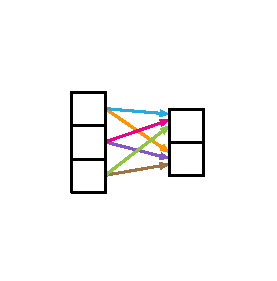
\includegraphics[height=3.0cm]{fig/content/intro/simpleNeuralNetwork/fcn.pdf}}
\subfigure[Convolutional]{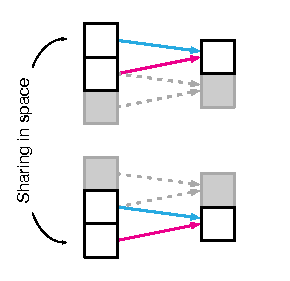
\includegraphics[height=3.0cm]{fig/content/intro/simpleNeuralNetwork/cnn.pdf}}
\subfigure[Recurrent]{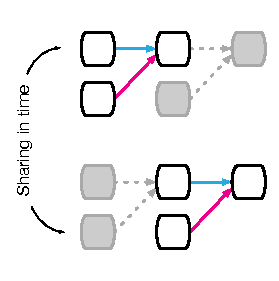
\includegraphics[height=3.0cm]{fig/content/intro/simpleNeuralNetwork/rnn.pdf}}
\caption{Simplified representation of some neural networks models ~\cite{Battaglia_2018}}

\label{fig:img1}
\end{figure}

Recently, between 2017 and 2018, papers ~\cite{Battaglia_2018, Gilmer_2017, Wang_2018} describing generalized graph prediction algorithms were published. These would provide a framework for predicting, with some acceptable error, output graphs given input graphs. Applications of these solutions varies from modelling molecular structures in Chemistry to Corpuscular Mechanics, and Community Studies.

In 2019, January 2nd a broad review ~\cite{Zhou_2019} of the main graph networks algorithms was carried out confirming that the Graph Nets’ approach ~\cite{Battaglia_2018} generalizes the Message Passing Neural Network ~\cite{Gilmer_2017} and Non Local Neural Network ~\cite{Wang_2018}, which by themselves were generalizing a lot of other methods. Some of those methods will be further detailed in the next section. This review presents the three cited algorithms. 


\subsection{Invariant Networks}

Given a graph $G = (V, A)$ consisting of $n$ nodes $V$ and values $A$ attached to its edges (in this case, an edge is an ordered subset of the nodes V).

When constructing a functional relation $f(A^l) \approx T^l$, where $f$ is a neural network and $T^l$ are the corresponding targets, if $f$ is order invariant, then it should produce the same output regardless of the node numbering used to encode $A$.

For example: Given an arbitrary adjacency matrix $A = A \in \mathds{R}^{n \times n}$, representing the graph. For an arbitrary permutation matrix P, the function f is order invariant if it satisfies $f(P^T A P) = f(A)$.

Since the neighborhood aggregation approach is as powerful as the Weisfeiler-Lehman graph isomorphism test ~\cite{Xu_2018}, we conjectured that the the Graph Nets’ approach would not be order invariant which would reflect in limitations on the algorithms’ performance when dealing with copies of a graph but permuted in representation. 